% !Mode:: "TeX:UTF-8"
%!TEX program  = xelatex

%\documentclass[bwprint]{cumcmthesis}
\documentclass[withoutpreface,bwprint]{cumcmthesis} %去掉封面与编号页

\title{太阳影子定位}
\tihao{A}
\baominghao{201723003002}
\schoolname{电子科技大学}
\membera{卫佳杰}
\memberb{谢沁余}
\memberc{任彦璟}
\supervisor{覃思义}
\yearinput{2017}
\monthinput{09}
\dayinput{01}

\begin{document}
 \maketitle
\begin{abstract}
\par 本文建立了通过在特定时间段太阳影子的变化确定拍摄直杆所在地点与日期的“太阳影子定位”模型,最后对视频进行图像处理后,确定了视频拍摄的地点和日期。
\par 第一问中,本文首先分析了直杆长度、拍摄日期、一天中的时间变化、和纬度对太阳下影子长度的影响关系。之后通过地理学知识确定了赤纬角、太阳高度角、时角、太阳方位角和直杆所在纬度值的内在关系。最终得出在2015年10月22日北京时间9:00-15:00天安门广场3米高的直杆的太阳影子长度变化图像。
\par 第二问中,基于建立对直杆影长进行二次拟合确定杆所在的经度位置的模型和“最小二乘”的最优化方法确定直杆所在的纬度的模型,得到附件一中直杆数据测量位置大约为海南省东方市。
\par 第三问中,基于建立“最小二乘”的最优化方法确定太阳赤纬赤尾角的模型,计算物体所在纬度,并通过第二问中的确定物体所在经度模型得出附件二中当物体的杆高为0.61米时, 直杆位于南纬 45 度 9 分 45 秒 东经 71 度 53 分 10 秒,拍摄时间为6 ⽉ 22 ⽇或 12 ⽉ 22 ⽇;当杆高为0.75米时,直杆位于北纬 52 度 17 分 17 秒 东经 71 度 53 分 10 秒拍摄时间为 6 ⽉ 22 ⽇或 12 ⽉ 22 ⽇.附件三中当物体的杆高为0.61米时, 直杆位于南纬 19 度 9 分 45 秒 东经 71 度 53 分 10 秒,拍摄时间为6 ⽉ 22 ⽇或 12 ⽉ 22 ⽇;当杆高为0.75米时,直杆位于北纬 19 度 30 分 10 秒 东经 71 度 53 分 10 秒,拍摄时间为 6 ⽉ 22 ⽇或 12 ⽉ 22 ⽇。
\par 第四问中,本文需要通过灰度化、⼆值化、缩放等⽅法对视频进⾏处理,采集其中直杆长度与影⼦长度的⽐例关系,通过图像获取到直杆与影⼦长度的⽐例关系后再使⽤第⼆、第三问中建⽴的模型进⾏计算。最终得到在已知拍摄日期的情况下,直杆所在的位置为南纬 0 度 1 分 17 秒,东经 124 度 17 分 24 秒。未知拍摄日期的情况下,直杆位于南纬 40 度 30 分 11 秒 东经 113 度 37 分 30 秒,拍摄时间为7 ⽉ 11 ⽇或者位于北纬 40 度 30 分 5 秒 东经 113 度 37 分 30 秒,拍摄日期为1 ⽉ 26 ⽇。

\keywords{二次拟合\quad 最小二乘法 \quad 最优化方法 \quad 灰度处理}
\end{abstract}

\tableofcontents
\newpage

\section{问题重述}

\par 如何确定视频的拍摄地点和拍摄日期是视频数据分析的重要方面,太阳影子定位技术就是通过分析视频中物体的太阳影子变化,确定视频拍摄的地点和日期的一种方法。因此,有以下四个问题:

\begin{enumerate}
	\item 建立影子长度变化的数学模型,分析影子长度关于各个参数的变化规律,并应用你们建立的模型画出2015年10月22日北京时间$9:00-15:00$之间天安门广场(北纬39度54分26秒,东经116度23分29秒)3米高的直杆的太阳影子长度的变化曲线。
	\item 根据某固定直杆在水平地面上的太阳影子顶点坐标数据,建立数学模型确定直杆所处的地点。将你们的模型应用于附件1的影子顶点坐标数据,给出若干个可能的地点。
	\item  根据某固定直杆在水平地面上的太阳影子顶点坐标数据,建立数学模型确定直杆所处的地点和日期。将你们的模型分别应用于附件2和附件3的影子顶点坐标数据,给出若干个可能的地点与日期。
	\item 附件4为一根直杆在太阳下的影子变化的视频,并且已通过某种方式估计出直杆的高度为2米。请建立确定视频拍摄地点的数学模型,并应用你们的模型给出若干个可能的拍摄地点。拍摄日期未知时能否根据视频确定出拍摄地点与日期。
\end{enumerate}

\section{问题分析}

\par 如何确定视频的拍摄地点和拍摄日期是视频数据分析的重要方面,太阳影子定位技术就是通过分析视频中物体的太阳影子变化,确定视频拍摄的地点和日期的一种方法。
\subsection{影子长度变化分析}

\par 依据地理学知识我们知道影子的长度是与直杆的长度、太阳直射点所在的纬度位置、物体所在的纬度位置、一天中的时刻有关的。我们采用控制变量的方法,建立影子长度关于各个参数的变化规律模型。并应用建立的模型可以得出具体地点,具体时间段的,长度固定直杆的影子长度变化曲线。

\subsection{直杆影子定位}

\par 当我们得到某固定直杆在水平地面上的太阳影子顶点在一段特定时间的坐标数据,与拍摄的日期。我们对各个时刻的影长利用最小二乘拟合、构建方程组求解该固定直杆所在的纬度的可能值与对应直杆长的可能值。通过地理知识我们得到一天中影长最短的时刻是当地的地方时正午12点,依据当地地方时与北京时间的关系,我们可以求出直杆所在的经度。因此直杆所在的经纬度便可以确定下来。
\subsection{未知日期条件下直杆影子定位}
\par 当我们得到某固定直杆在水平地面上的太阳影子顶点在一段特定时间的坐标数据,但是并不知道拍摄的日期。我们利用最小二乘拟合、构建方程组求解太阳的赤纬角,通过赤纬角我们可以的到拍摄日期的可能值与对应杆长的可能值。依据我们确定出的赤纬角与直杆长度,可以计算得到该直杆所在可能的纬度值。计算经度可以用第二问计算经度的方法计算。因此直杆拍摄的地理位置和拍摄日期得以确定。
\subsection{视频拍摄地点分析}
\par 通过图像视频处理的相关技术,我们可以从视频中得到固定直杆在水平地面上的太阳影子顶点在一段特定时间的坐标数据。运用第二问和第三问的模型进行求解。
\section{基本假设}
\begin{enumerate}
	\item 假设地球为均匀球体,且地球绕太阳公转轨道为圆形。
	\item 忽略太阳光线在大气中的折射。
	\item 直杆垂直于地面放置。
	\item 假设一天中太阳直射点维度不变。
	\item 忽略相机透镜造成的形变。
\end{enumerate}
\newpage
\section{符号说明}

\begin{table}[!h]
\centering
\begin{tabular}{ccc}
\toprule
 \makebox[0.2\textwidth][c]{符号}	&  \makebox[0.5\textwidth][c]{意义} &  \makebox[0.2\textwidth][c]{单位} \\ \midrule
 $\alpha$	& 太阳方位角  &度\\ 
 $H$	    & 太阳高度角  &度\\ 
 $\varphi$	& 太阳赤纬角  &度\\ 
 $t$	& 太阳时角  &度 \\ 
 $\gamma$   & 经度&度\\
 $\theta$	& 纬度&度\\
 $L$		& 直杆长度&m\\
 $L_S$		& 影子长度&m\\
 $ST$       & 真太阳时\\
 $\Delta t$ & 于北京时间的时差\\
\bottomrule 
\end{tabular}
\end{table}
\newpage
\section{影子长度变化的分析}
\subsection{问题分析}
对于问题一,为了描述直杆影子长度变化的过程。首先以直杆向上方向为Z轴正方向建立空间直角坐标系。为了降低分析难度,在假设的前提下,假定地球为球坐标原点,且固定不动,令太阳在圆轨道上绕地球转转。通过对两个坐标系中的相关角度、向量的关系进行分析,得出影响直杆影子长度的各项参数,得到直杆影子端点在坐标系中的位置表达式。最终可由此求出直杆影子长度随各个参数变化的规律。
\subsection{模型建立}
\par 直杆的影子是由于太阳对直杆的照射产生的,且由几何关系可知,杆长$L$、影长$L_S$、太阳高度角$H$之间存在关系$L_S = \frac{L}{tan H}$(如图(\ref{fig:q1-1})所示)。通过查阅相关文献\upcite{q1-1},太阳高度角与赤纬角、时角相关,通过这些相关变量建立直杆影子长度变化模型。
\subsubsection{坐标系建立}
\par 根据假设,视太阳光线为平行光,以直杆所在地点的正东方向为$x$轴,以正北方向为$y$轴,以直杆直立即垂直于$oxy$平面的方向为z轴,建立空间直角坐标系,得到直杆在$oxy$平面的投影与光线的位置关系,如下图(\ref{fig:q1-1})所示,其中$H$为太阳高度角,$L$为直杆长度,$L_S$为影子长度。
\begin{figure}[h]
\small
\centering
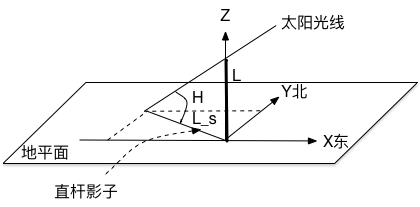
\includegraphics[width=12cm]{直角坐标系.png}
\caption{直杆处空间直角坐标系建立} \label{fig:q1-1}
\end{figure}
\par 对于太阳高度角的计算,给出时角坐标系(如图(\ref{fig:q1-2})所示)的定义。
\begin{figure}[h]
\small
\centering
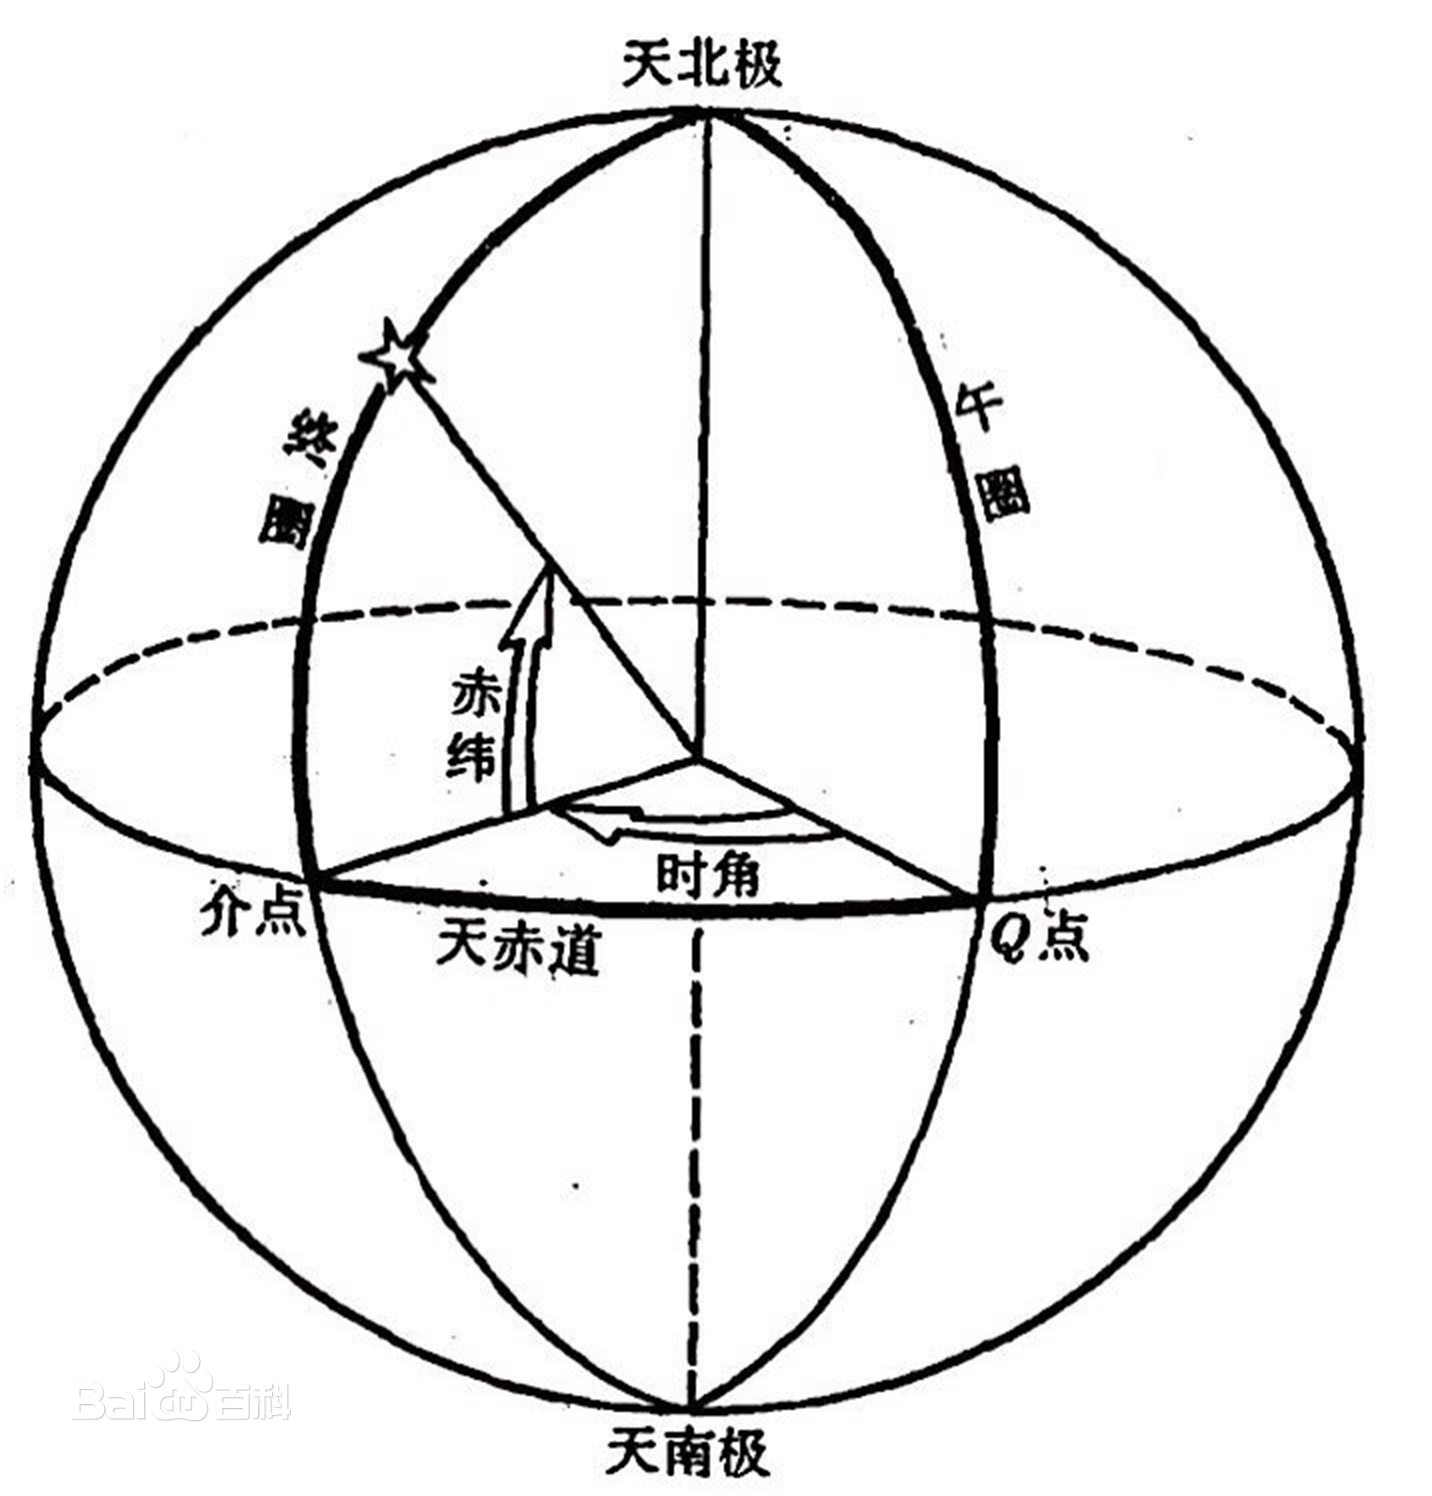
\includegraphics[width=10cm]{时角坐标系.png}
\caption{地球时角坐标系建立} \label{fig:q1-2}
\end{figure}
\par 时角坐标系又称第一赤道坐标系。时角坐标系的基本要素如下:
\begin{enumerate}
	\item 基本大圆:天赤道
	\item 坐标原点:天赤道和测者子午圆在午半圆的交点
	\item 坐标:纬度为赤纬,经度为时角\upcite{时角}
\end{enumerate}
\subsubsection{赤纬角\upcite{赤纬角}}
如图(\ref{fig:q1-2})所示,太阳赤纬角指地球赤道平面与太阳和地球中心连线之间的夹角,也称为黄赤交角。赤纬角存在缓慢的变化,范围在$22°00′$到$24°30′$,变化的周期约为$4.1×10^4$年。赤纬角计算可通过如下公式(\ref{chiweijiaojisuan})进行计算,其中$t_{year}$是1900年起算的儒略年数。

\begin{equation}
\label{chiweijiaojisuan}
	\varphi = 23.45^osin((N-80.25)\dot(1-\frac{N}{9500}))	
\end{equation}

\subsubsection{时角\upcite{时角}}

\par 单位时间地球自转的角度定义为时角,规定正午时角为$0^o$,上午时角为负值,下午时角为正值。每$4$分钟的时角度数为$1^o$时角可以通过如下公式(\ref{shijiaojisuan})进行计算,其中$t$为时角,$t_h$为当前时间(小时为单位)。

\begin{equation}
	\label{shijiaojisuan}
	t = 15^o\times (t_h-12)
\end{equation}

\par 地方时与标准时之间转换关系如下公式(\ref{biaozhunshi})所示,其中$\gamma$为直杆所在地的经度,$\gamma_0$为北京时间的定义下的经度(即东经$120^o$),$E_p$为时差。

\begin{equation}
\label{biaozhunshi}
	t_{Beijing} = t_{Difang}+4(\gamma_0 - \gamma)+E_p
\end{equation}

\subsubsection{太阳高度角\upcite{高度角}}
太阳高度角指太阳光线的入射方向和地平面之间的夹角,专业上讲太阳高度角指太阳光线与通过该地与地心相连的地表切线的夹角。太阳高度角可通过如下公式(\ref{gaodujiao})进行计算。
\begin{equation}
	\label{gaodujiao}
	sin(H) = sin(\theta)sin(\varphi)+cos(\theta)cos(\varphi)cos(t)
\end{equation}

\subsubsection{影长计算模型}
通过上述各个角度转换关系,确定以下方程组(\ref{moxingyi}),建立影长计算模型。

\begin{equation}
\label{moxingyi}
\left\{  
  	\begin{array}{lr}  
  		L_S = \frac{L}{tan H} \\ 
  		sin(H) = sin(\theta)sin(\varphi)+cos(\theta)cos(\varphi)cos(t)\\
  		
  		\varphi = 23.45^osin((N-80.25)\dot(1-\frac{N}{9500}))	\\  
  		t = 15^o\times (t_h-12)\\
		t_{Beijing} = t_{Difang}+4(\gamma_0 - \gamma)+E_p\\
		    
	\end{array}  
\right.  
\end{equation}



\subsection{模型求解}

\subsubsection{相关变量影响分析}
通过分析,影响直杆影子长度的4个主要参数为:纬度$\gamma$、直杆长度$L$、日期、时间。如下图(\ref{fig:q1-2-1},\ref{fig:q1-2-2},\ref{fig:q1-2-3},\ref{fig:q1-2-4})所示为直杆影子长度在其他参数不变的条件下,分别随前述一个个参数变化的结果。

\begin{figure}[!htbp]  
\begin{minipage}[t]{0.5\textwidth}
\centering  
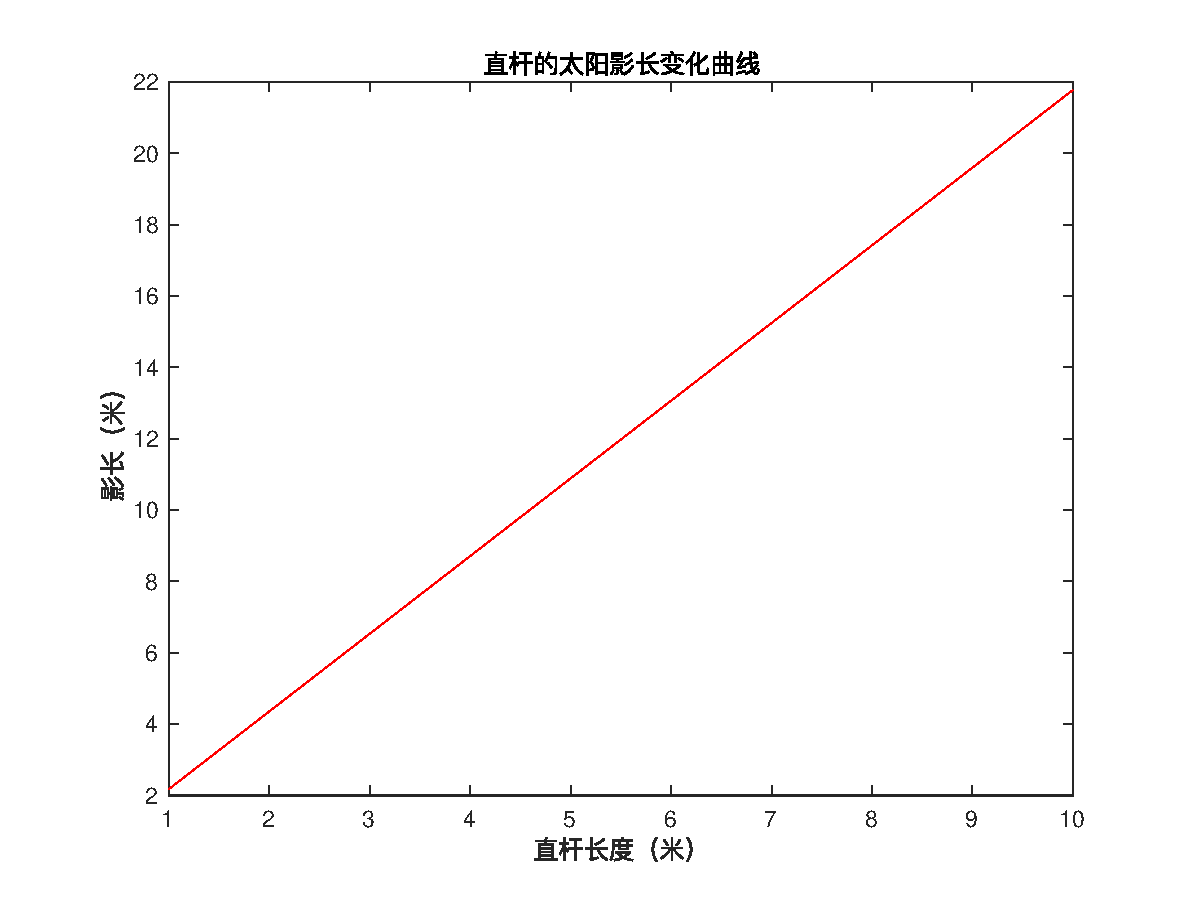
\includegraphics[width=\linewidth]{q1-zhigan.eps}
\caption{影长随直杆长度变化的结果} \label{fig:q1-2-1}\end{minipage}
\hspace{1ex}
\begin{minipage}[t]{0.5\textwidth}  
\centering  
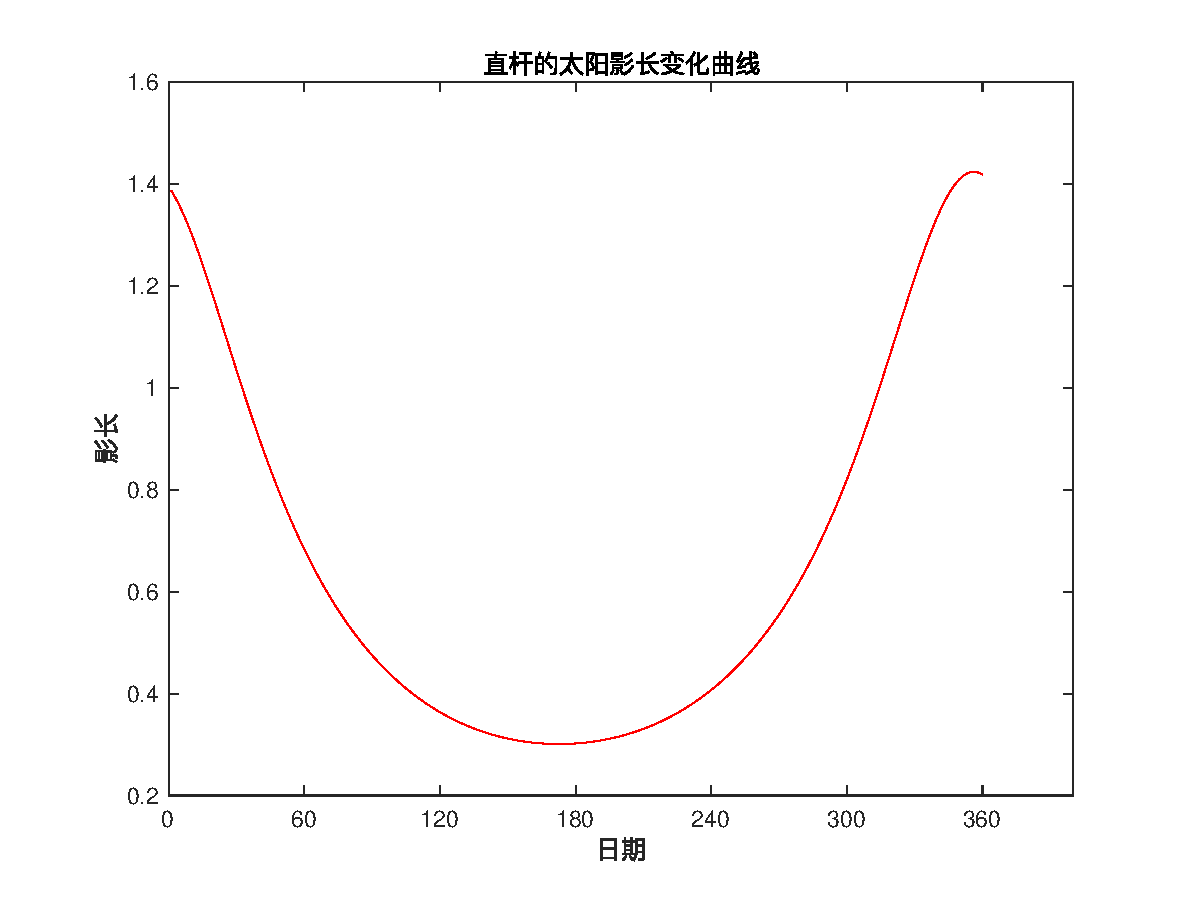
\includegraphics[width=\linewidth]{q1-date.eps}
\caption{影长随日期变化的结果} \label{fig:q1-2-2}
\end{minipage}  
\end{figure} 

\begin{figure}[!htbp]  
\begin{minipage}[t]{0.5\textwidth}
\centering  
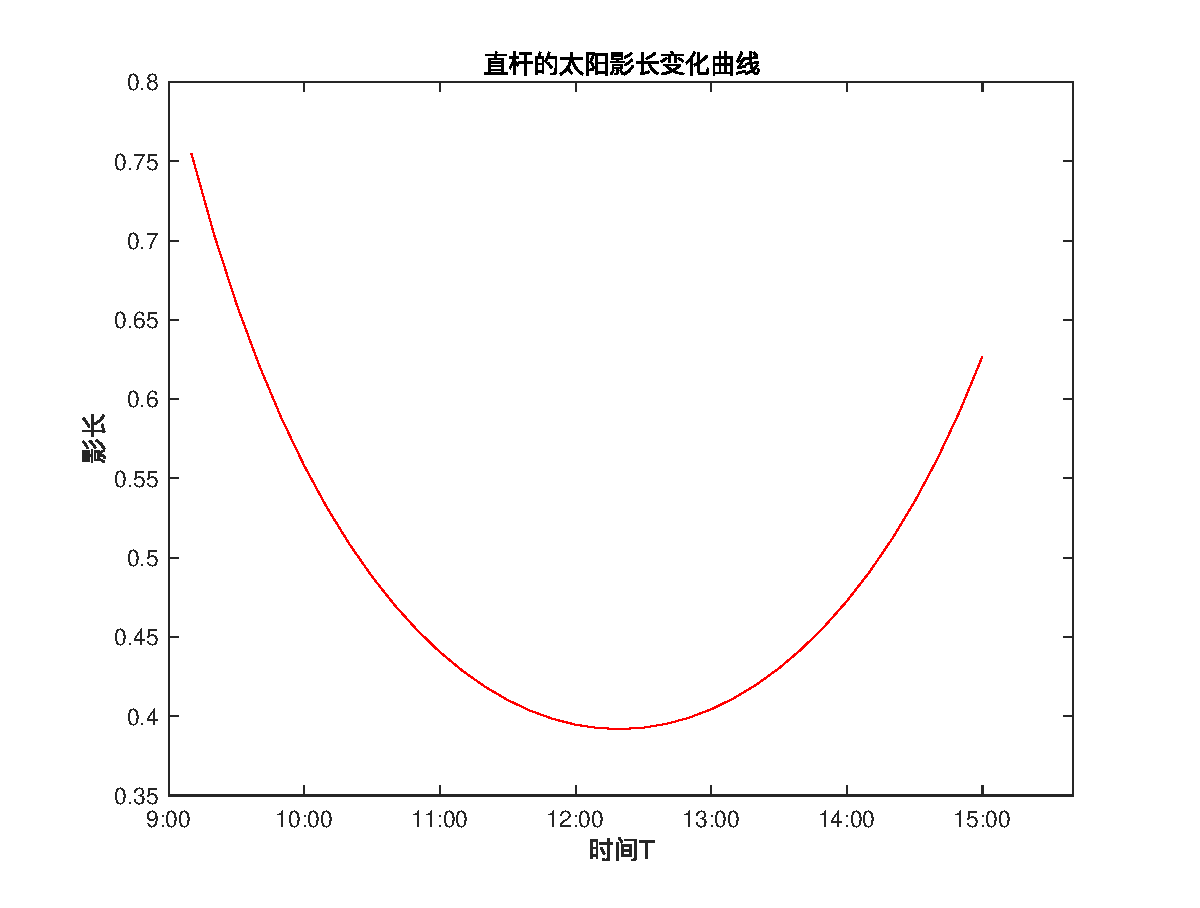
\includegraphics[width=\linewidth]{q1.eps}
\caption{一天内影长随时间变化的结果} \label{fig:q1-2-3}\end{minipage}
\hspace{1ex}
\begin{minipage}[t]{0.5\textwidth}  
\centering  
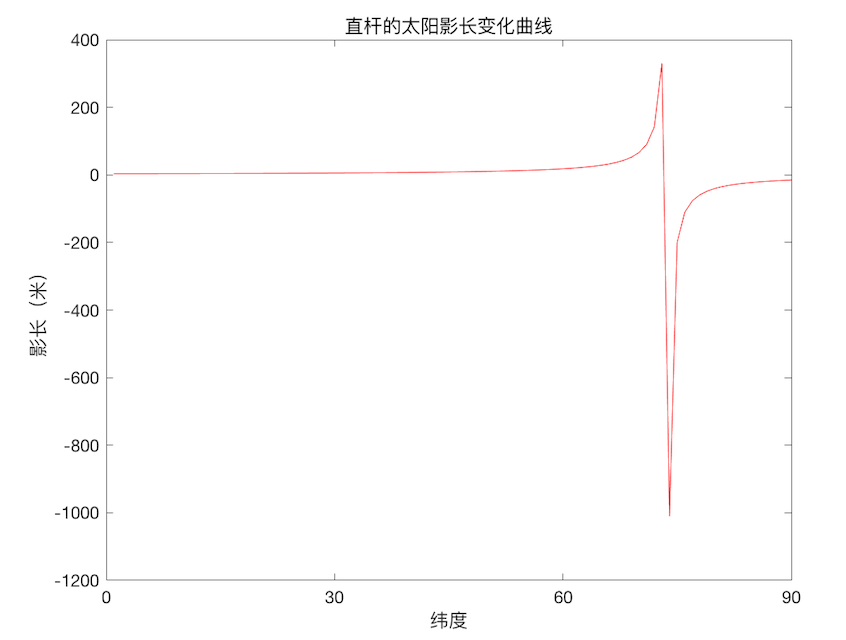
\includegraphics[width=\linewidth]{q1-weidu.png}
\caption{影子长度随纬度的变化} \label{fig:q1-2-4}
\end{minipage}  
\end{figure} 





\par 如上图(\ref{fig:q1-2-1})所示,为固定地点为天安门广场(北纬39度54分26秒,东经116度23分29秒),日期为2015年10月22日,时间为北京时间9:00-15:00之间,将直杆长度在$1\sim10$米之间变动的影子长度变化曲线。

\par 如上图(\ref{fig:q1-2-2})所示,为固定地点为天安门广场(北纬39度54分26秒,东经116度23分29秒),直杆长度为3米,时间为北京时间9:00-15:00之间,将日期在2015年1月1日和12月31之间变动的影子长度变化曲线。
\par 如上图(\ref{fig:q1-2-3})所示,为固定地点为天安门广场(北纬39度54分26秒,东经116度23分29秒),日期为2015年10月22日,时间在北京时间9:00-15:00之间变动的影子长度变化曲线。
\par 如上图(\ref{fig:q1-2-4})所示,为固定日期为2015年10月22日,时间为北京时间9:00-15:00之间,直杆长度为3米,经度为东经116度23分29秒时将纬度由0度至90度变动时影子长度变化曲线。

\par 由影长随各参数变化的计算结果,可知:当其它参数一定时,影子长度与直杆长度成线性关系,与日期、时间和维度呈非线性关系,并且与后三者存在周期性。

\subsubsection{直杆影子长度变化分析}

通过计算得到不同时刻下影子长度变化曲线如图(\ref{fig:q1-ans})所示,
为2015年10月22日北京时间9:00-15:00之间天安门广场(北纬39度54分26秒,东经116度23分29秒)3米高直杆的影子长度变化。
\begin{figure}[h]
\small
\centering
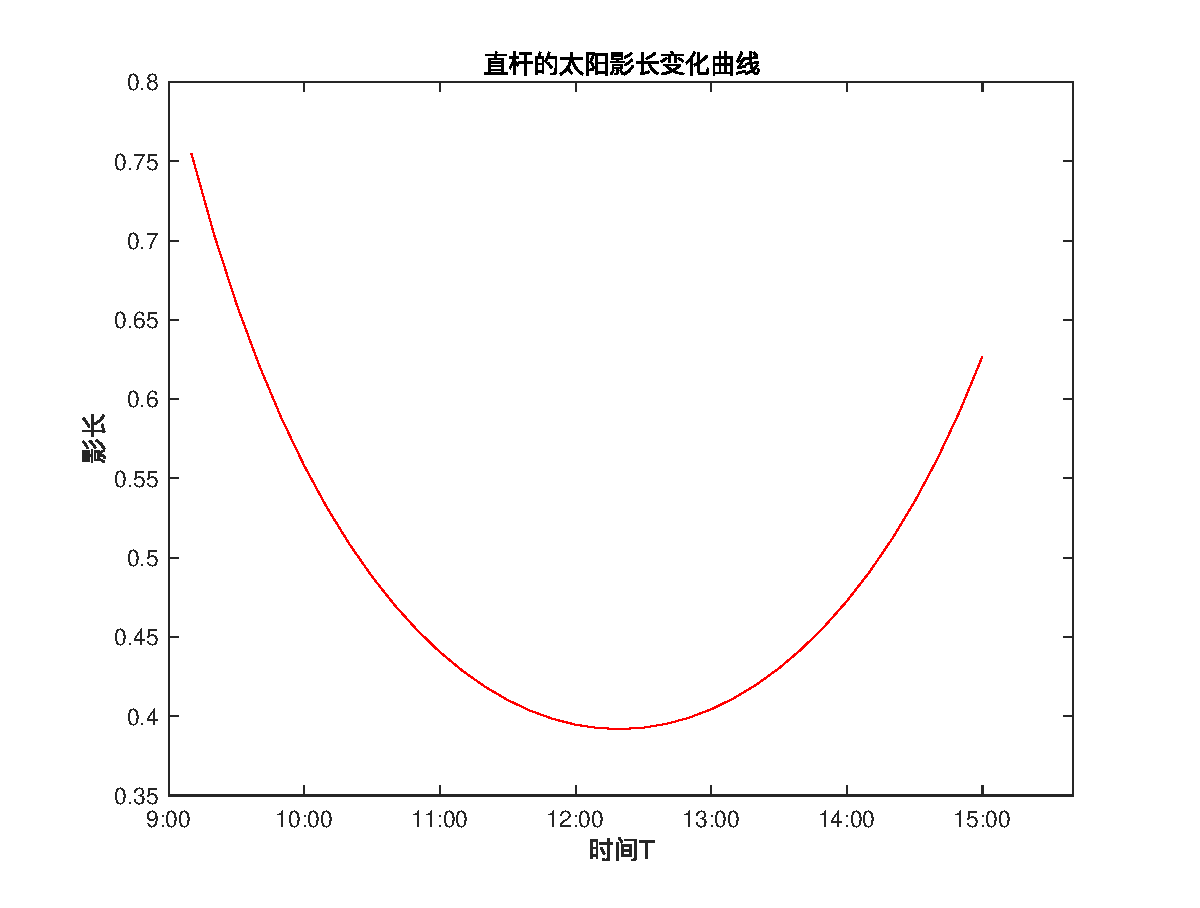
\includegraphics[width=12cm]{q1.eps}
\caption{直杆影子长度变化曲线} \label{fig:q1-ans}
\end{figure}



\newpage
\section{直杆影子定位}
\subsection{模型建立}
第二问中,需要通过影子坐标确定直杆的经纬度。由第一问的分析可以知道影子长度随时间大致呈现一个二次曲线。本题中以北京时间为横坐标影长为纵坐标,先进行二次拟合,最低点横坐标可近似认为当地正午所对应的北京时间。根据正午的北京时间可计算出杆所在经度的估计值。将估计值正负5度作为经度的搜索范围,-90度到90度作为纬度的搜索范围,通过基于最小二乘的最优化方法求解直杆所在的经纬度的模型确定杆所在的经纬度。搜索分两次进行,先用大步长1度确定一个经纬度,在该经纬度正负1度的范围内再用小步长0.1度进行搜索。最终得到直杆的经纬度和可能的地点。


\subsubsection{基于对“杆的影长”二次拟合确定杆所在经度的范围的模型}


\par 地球自转一周,转过360度,同时经过1440分钟,因此,地球自转角速度为4分钟/度。由于运动的相对性可知,太阳相对地球的转动速度为4分钟/度。

\par 由地理学的相关知识可得,如图(\ref{fig:q2-1})所示,通过英国伦敦格林尼治天文台原址的那一条经线定为0°经线,也叫本初子午线,从这条线往东(向右)为东经,度数逐渐增大到180°。从0°经线往西(向左)为西经,度数也逐渐增大到180°,东西180°经线是同一条经线,越向东的地方的地方时越领先。经度每向东1度,地方时增加4分钟。以$[\gamma -5, \gamma +5]$作为经度的搜索范围。

\begin{figure}[h]
\small
\centering
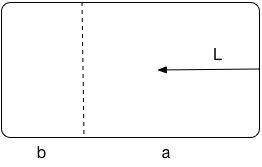
\includegraphics[width=12cm]{q2-1.png}
\caption{经线定义} \label{fig:q2-1}
\end{figure}


北京时间是指的是东经120度的地方时。通过第一问的分析可知,正午直杆的影子长度随一天时间的变化先减小后增大,变化过程是类抛物线图形,当当地的地方时为正午12:00时,直杆的影长最短。通过对附件一的数据进行二次拟合,对该二次函数求出影长最小值所对应的时间为该地区的北京时间,可通过公式(\ref{difangshi})计算得到直杆所在位置的经度,其中$\gamma$为经度,$\Delta t$为与北京时间的时间差。
 
\begin{equation}
	\label{difangshi}
	\gamma = 120 -\frac{\Delta t}{4}
\end{equation}

\subsubsection{基于“最小二乘”的最优化方法求解直杆所在的纬度的模型}

\begin{equation}
	\label{q2-1-min}
	min \frac{1}{N} \sum\limits_{i=1}^{N}(L_i - \bar{L})^2
\end{equation}
\begin{equation}
\label{moxingerguihua}
s.t.\left\{  
  	\begin{array}{lr}
  	106^o \leqslant \alpha \leqslant 116^o\\
  	-90^o \leqslant \theta \leqslant 90^o\\  
	\end{array}  
\right.  
\end{equation}

其中任一时刻杆长的计算方法如下公式(\ref{moxinger})所示

\begin{equation}
\label{moxinger}
\left\{  
  	\begin{array}{lr} 
  		\Delta t = \frac{\alpha - 120^o}{15^o}\\
  		ST = t_{beijing} + \Delta t\\
  		t = 15\times (ST - 12)\\
  		\varphi = 23.45 sin \frac{2\pi(284+m)}{365}\\
  		sin(H) = sin(\theta)sin(\varphi)+cos(\theta)cos(\varphi)cos(t)\\
  		L_{si} = \sqrt{x_i^2+y_i^2}\\
  		L_i = L_{si}tan(H)\\
  		\bar{L}_i  = \frac{1}{d_i}\sum\limits_{i=1}^{d_i} L_i\\
	\end{array}  
\right.  
\end{equation}

\par 我们建⽴在对杆⾼误差的最⼩平⽅和条件下确定的经纬度值计算模型,如公式组(\ref{moxingerguihua}) 所⽰。


\begin{enumerate}
	\item 第一个公式用来计算该地与东经120度(北京时间)的时差
	\item 第二个公式计算出该地的真太阳时
	\item 第三个公式计算出时⾓,在地球上,同⼀时刻,对同⼀经度,不同纬度的⼈来说, 太阳对应的时⾓是相同的。单位时间地球⾃转的⾓度定义为时⾓$\omega$,规定正午时⾓为0,上午时⾓为负值,下午时⾓为正值。地球⾃转⼀周360度,对应的时间为24⼩时,即每⼩时相应的时⾓为15度。
	\item 第四个公式是⾚纬⾓公式$\varphi$\upcite{赤纬角},描述的是由于地球有黄道交⾓,所以地球在绕太阳运动的时候太阳的直射点会在南北回归线间做循环往复的移动,⽽对于每天太阳直射点的纬度位置由第⼆个公式可见。
	\item 第五个公式是建⽴的太阳⾼度⾓H与太阳⾚尾⾓、物体所在的纬度值、和太阳时⾓$t$的关系\upcite{时角}。
	\item 第六个公式描述的是投影平⾯内影长$L_s$的计算公式。
	\item 第七个公式描述的杆⾼$L$与影长$L_s$的关系。 
	\item 第八个公式描述的是对每⼀时刻的杆的长度求均值的过程。 
由于杆的长度在各种情况下求出都应该为定值,⽬标函数(\ref{q2-1-min})使每⼀时刻 求出的杆的长度误差的平⽅和最⼩,在约束条件下可解得经度值和纬度值。
\end{enumerate}

\par 由于杆的长度在各种情况下求出都应该为定值,目标函数(公式(\ref{q2-1-min}))使每一时刻求出的杆的长度误差的平方和最小,在约束条件下可解得纬度值。

\subsection{模型求解}
\subsubsection{经度范围的确定}
 对附件一先以时间为自变量,影子的长度为因变量进行二次拟合,如下图(\ref{fig:q2-jingdu})所示,当地正午为北京时间12时35分,并通过公式求得经度为东经111度1分21秒。以$[106°E, 116°E]$作为经度的搜索范围。

\begin{figure}[h]
\small
\centering
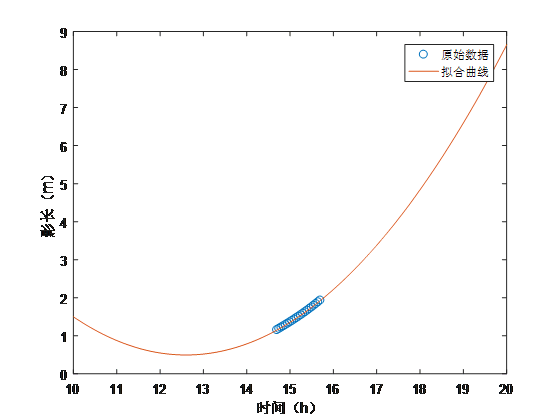
\includegraphics[width=12cm]{q2-jingdu.png}
\caption{经度求解结果} \label{fig:q2-jingdu}
\end{figure}
 
\subsubsection{经纬度求解步骤及结果}
将$[106°E, 116°E]$作为经度的搜索范围,$[90°S, 90°N]$作为纬度的搜索范围,先以1度为步长通过基于最小二乘的最优化方法求解直杆所在的经纬度的模型确定杆所在的经纬度,结果如下表(\ref{步长为1度搜索})所示:

\begin{table}[!htbp]
\centering
\caption{步长为1度搜索}
\label{步长为1度搜索}
\begin{tabular}{cccc}
\toprule
经度&纬度&目标函数\\
\midrule
109E & 19N & 2.15E-08 \\
110E & 18N & 5.45E-07 \\
\bottomrule 
\end{tabular}
\end{table}

\par 可以看出,求解出的经纬度都非常接近,也说明方法的稳定性和合理性。

\par 将$[108°E, 110°E]$作为经度的搜索范围,$[18°N, 20°N]$作为纬度的搜索范围,再以0.1度为步长通过基于最小二乘的最优化方法求解直杆所在的经纬度的模型确定杆所在的经纬度,结果如下表(\ref{步长为0.1度搜索})所示:

\begin{table}[!htbp]
\centering
\caption{步长为0.1度搜索}
\label{步长为0.1度搜索}
\begin{tabular}{cccc}

\toprule
经度&纬度&目标函数\\
\midrule
108.6E&19.3N&4.01E-09\\
\bottomrule 
\end{tabular}
\end{table}

最终查询结果为海南省东方市。

\newpage
\section{未知日期条件下直杆影子定位}
\subsection{根据影子的顶点坐标确定直杆的可能的位置与观测时间的多目标优化模型}


通过前一问的分析我们可以知道对于某一段特定的时间和确定的日期和直杆的经纬度位置决定直杆的影子的长度变化以及影子方向角度的变化。与前一问相同,我们建立不同位置,不同日期的太阳影子长度与实测影长的优化模型。本问中我们将搜索范围进行扩大,将全球与全年作为搜索范围,在满足约束条件的情况下,我们给出直杆影长与实测影长变化相差较小的直杆所在的经纬度位置与日期。

\subsubsection{建模前准备}
题目中附件二、附件三给出的测量时间段分别是北京时间12:41-13:41与北京时间13:09-14:09。每隔三分钟对直杆影子的顶点坐标进行测量一次,分别进行了21次的测量。

测量出的影长用$L_{s(i)}$表示;测出的方位角用$\alpha_{\theta(i)}$表示;对全球任意一点(经纬度)第i个时刻所对应的影子长度用$L_{y\theta (i)}$表示;对全球任意一点(经纬度)第i个时刻所对应的方位角用$\alpha_{y \theta (i)}$表示。

\subsubsection{多目标的优化模型建立}
对于通过影子顶点坐标数据确定直杆所处地点和日期的问题,我们给出所建立的多目标优化模型:

\begin{equation}
	\label{q3-1-min}
	min \sum\limits_{i=1}^{21}(L_{y\theta(i)} - L_{S(i)})^2 \quad min \sum\limits_{i=1}^{20}(\alpha_{(i)} - \alpha_{o(i)})^2 
\end{equation}

\begin{equation}
\label{moxingsan}
s.t.
\left\{  
  	\begin{array}{lr}  
  		-180^o \leqslant \gamma \leqslant 180^o\\
  		-90^o \leqslant \theta \leqslant 90^o\\
  		0 \leqslant L \leqslant 6m\\
  		0 < N \leqslant 365\\
	\end{array}  
\right.  
\end{equation}

在上述优化模型中,$\gamma$为经度、$\theta$为维度、$L$为直杆实际长度、日期$N$为决策变量。在优化目标中,$L_{\alpha \varphi (i)}$的计算公式如下公式(\ref{jisuanyouhua})所示:
\begin{equation}
\label{jisuanyouhua}
\left\{  
  	\begin{array}{lr}  
  		L_{\gamma \theta (i)} = L \dot cot[arcsin(sin\theta sin\varphi + cos\theta cos\varphi cost)]\\
  		\varphi = 23.45^o sin((N-80.25)(1-\frac{N}{9500}))\\
  		t = 15^o\times (t_n -12)\\
	\end{array}  
\right.  
\end{equation}

其中$\alpha_{ y \theta(i)}$,计算公式为(\ref{yijisuan}):
\begin{equation}
	\label{yijisuan}
	\alpha_{ y \theta(i)} = \mid \alpha_{S1} - \alpha_{Si}  \mid 
\end{equation}

\subsection{模型求解}
\subsubsection{经度计算}
对附件二先以时间为自变量,影子的长度为因变量进行二次拟合,如图(\ref{fig:q3-fu2})所示,当地正午为北京时间15时12分,并通过公式求得经度为东经71度53分10秒。
\begin{figure}[h]
\small
\centering
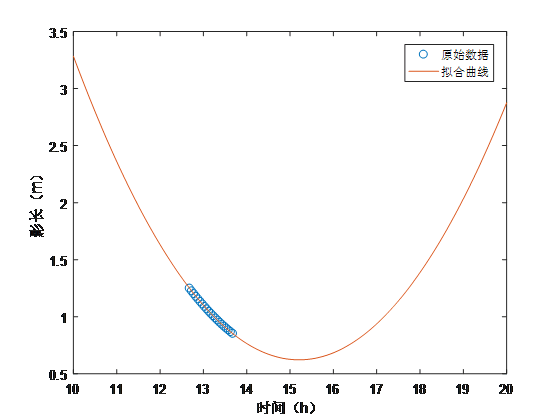
\includegraphics[width=12cm]{q3-fu2.png}
\caption{附件二经度求解结果} \label{fig:q3-fu3}
\end{figure}

对附件三用相同的方法,如图(\ref{fig:q3-fu3})所示,求得经度为东经108度57分36秒。

\begin{figure}[h]
\small
\centering
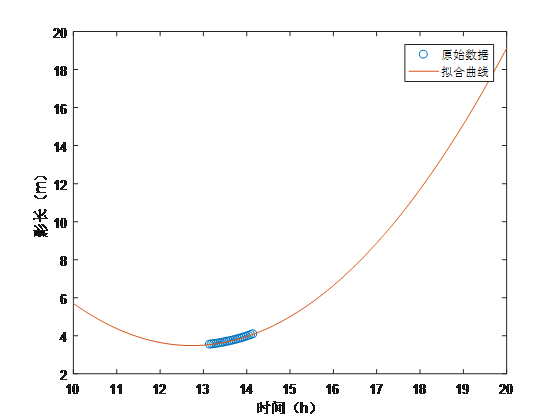
\includegraphics[width=12cm]{q3-fu3.png}
\caption{附件三经度求解结果} \label{fig:q3-fu3}
\end{figure}

\subsubsection{纬度计算}

将上述的方程带入matlab求解,可以得到在不同纬度值与目标函数的大小的离散关系,如图(\ref{fig:q3-weidu})所示:

\begin{figure}[h]
\small
\centering
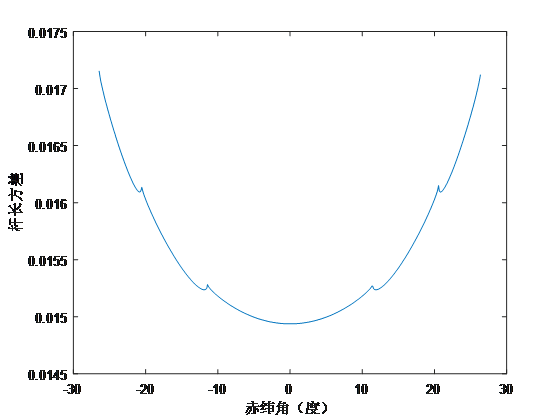
\includegraphics[width=12cm]{q3-weidu.png}
\caption{维度求解结果} \label{fig:q3-weidu}
\end{figure}


通过图(\ref{fig:q3-weidu}),可以得到在目标函数值在南纬90度到北纬90度的范围中先减小后增大。接下来用matlab通过取更小的步长0.01°,对可能会产生局部极小值的地方进行细分,并观察对应的纬度值。若通过21个数据计算出纬度波动不大,则可认为是直杆所在位置的纬度。


\subsubsection{最终求解结果}
通过模型解得直杆的相关数据如下表(\ref{q3-1经纬度求解结果},\ref{q3-2经纬度求解结果})所示。附件二结果对应实际地点如图(\ref{fig:q3-2-yingdu},\ref{fig:q3-2-yazhou})所示,分别位于印度洋与俄罗斯附近;附件二结果对应实际地点如图(\ref{fig:q3-3-yindu},\ref{fig:q3-3-yingduyang})所示,分别位于印度与印度洋中。
\begin{table}[!htbp]
\centering
\caption{附件二经纬度求解结果}
\label{q3-1经纬度求解结果}
\begin{tabular}{cccc}
\toprule
杆高(米)&纬度&经度 & 日期\\ 
\midrule
0.6112&南纬45度9分45秒&东经71度53分10秒&6月22日或12月22日\\
0.745&北纬52度17分17秒&东经71度53分10秒&6月22日或12月22日\\
\bottomrule 
\end{tabular}
\end{table}

\begin{table}[!htbp]
\centering
\caption{附件三经纬度求解结果}
\label{q3-2经纬度求解结果}
\begin{tabular}{cccc}
\toprule
杆高(米)&纬度&经度 & 日期\\ 
\midrule
0.6112&南纬19度9分45秒&东经71度53分10秒&6月22日或12月22日\\
0.745&北纬19度30分10秒&东经71度53分10秒&6月22日或12月22日\\
\bottomrule 
\end{tabular}
\end{table}


\begin{figure}[!htbp]  
\begin{minipage}[t]{0.5\textwidth}
\centering  
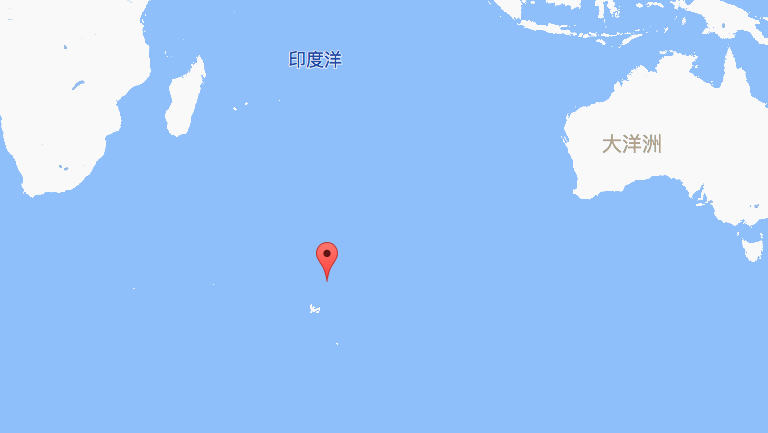
\includegraphics[width=\linewidth]{q3-2-yingdu.png}
\caption{地点一:印度洋中} \label{fig:q3-2-yingdu}\end{minipage}
\hspace{1ex}
\begin{minipage}[t]{0.5\textwidth}  
\centering  
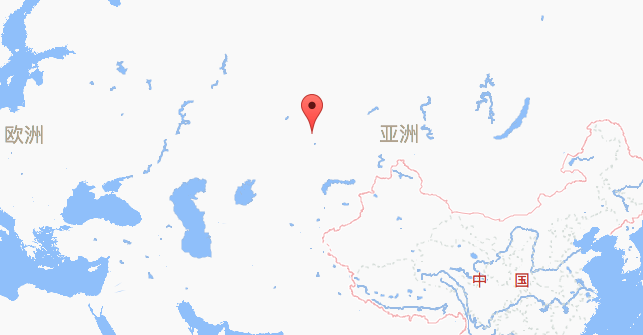
\includegraphics[width=\linewidth]{q3-2-yazhou.png}
\caption{地点二:俄罗斯} \label{fig:q3-2-yazhou}
\end{minipage}  
\end{figure} 


\begin{figure}[!htbp]  
\begin{minipage}[t]{0.5\textwidth}
\centering  
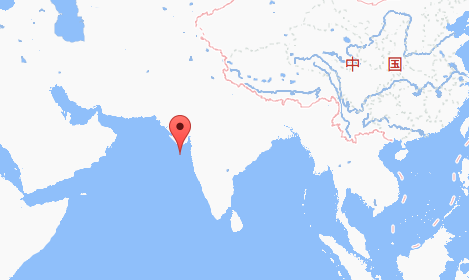
\includegraphics[width=\linewidth]{q3-3-yindu.png}
\caption{地点一:印度} \label{fig:q3-3-yindu}\end{minipage}
\hspace{1ex}
\begin{minipage}[t]{0.5\textwidth}  
\centering  
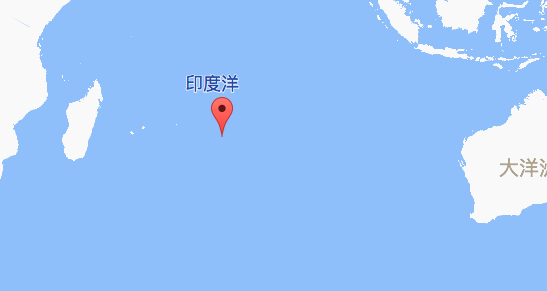
\includegraphics[width=\linewidth]{q3-3-yingduyang.png}
\caption{地点二:印度洋中} \label{fig:q3-3-yingduyang}
\end{minipage}  
\end{figure} 




\newpage
\section{视频拍摄地点分析}
\subsection{模型建立}
第四问中,首先需要通过灰度化、二值化、缩放等方法对视屏进行处理,采集其中直杆长度与影子长度的比例关系,通过图像获取到直杆与影子长度的比例关系后再使用第二、第三问中建立的模型进行计算。
\subsubsection{视频帧截取与灰度处理}
视频总长度为40分钟,按照附件二、附件三的形式,应当在附件四的视频中等时间间隔截取二十个数据点,即从中等间距截取二十帧图像。
在截取图像完成后,为了便于人工标定直杆、影子,因此将图像进行灰度处理。结果如图(\ref{fig:gray})所示。

\begin{figure}[h]
\small
\centering
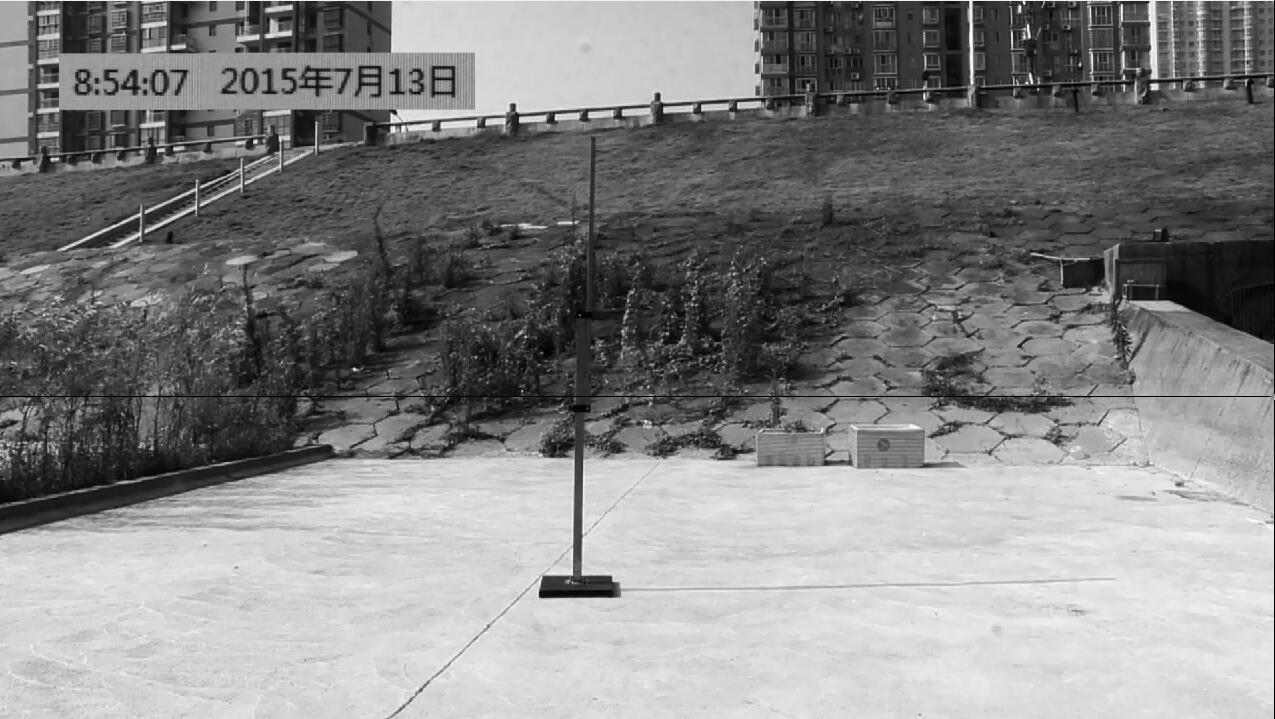
\includegraphics[width=12cm]{gray.jpg}
\caption{灰度处理结果} \label{fig:gray}
\end{figure}
\subsubsection{图像二值化处理与缩放}
图像二值化就是将图像上的像素点的灰度值设置为0或255,也就是将整个图像呈现出明显的黑白效果的过程。图像的二值化使图像中数据量大为减少,从而能凸显出目标的轮廓。便于影子坐标与长度的标定。结果如图(\ref{fig:rgb2})所示。

\begin{figure}[h]
\small
\centering
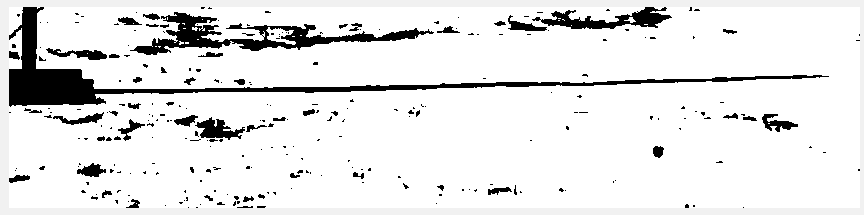
\includegraphics[width=12cm]{rbg2.png}
\caption{缩放与二值化结果} \label{fig:rgb2}
\end{figure}
\subsection{模型求解}

\subsubsection{已知时间}

时间为自变量,影子的长度为因变量进行二次拟合,绘图如下,当地正午为北京时间11时42分,并通过公式求得经度为东经124度17分24秒。
\begin{figure}[h]
\small
\centering
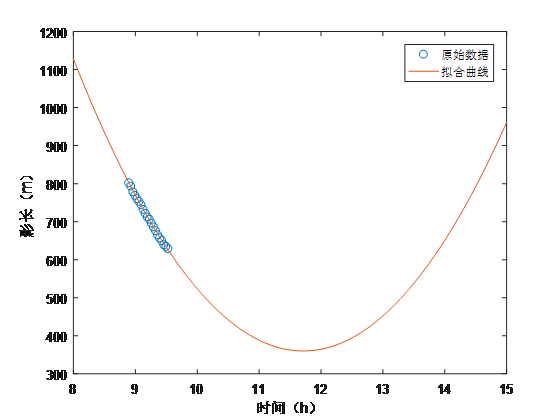
\includegraphics[width=12cm]{q4-jingdu.png}
\caption{经度求解结果} \label{fig:q4-jingdu}
\end{figure}

\par 杆长及影子的测量;杆长测4次后取平均,得到了2m杆长对应的长度663.4482个单位;影子的测量也通过截出的20帧画面结合之前描述方法实现。
\par 求解纬度时,应用问题二中的模型,将上述的方程带入matlab求解,可以得到在不同纬度值与目标函数的大小的离散关系。

\begin{figure}[h]
\small
\centering
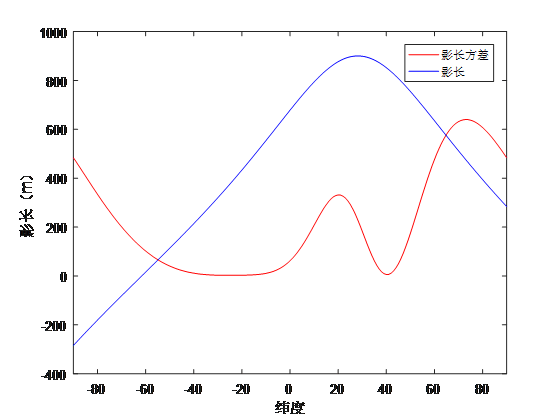
\includegraphics[width=12cm]{q4-weidu.png}
\caption{纬度求解结果} \label{fig:q4-weidu}
\end{figure}

\par 通过图(\ref{fig:q4-weidu}),可以得到在目标函数值在南纬90度到北纬90度的范围中会存在有两个极小值。但结合条件,杆长对应的长度为663.4482个单位,因而纬度范围被控制在北纬[-1°,0°],南纬[58°,59°]。而南纬[58°,59°]对应的影长方差远大于北纬[-1°,0°],因此只在北纬[-1°,0°]范围内用更小的步长0.01搜索,可认为计算的平均杆长与663.4482最接近的纬度值为直杆所在位置的纬度。最终平均杆长为663.4836个单位,纬度为南纬0度1分17秒。

\subsubsection{未知时间}
应用问题三中的模型将上述的方程带入matlab求解,可以得到在不同赤纬角与目标函数的大小的离散关系,解得对应的经纬度坐标。

\subsubsection{最终求解结果}
通过模型解得直杆的相关数据如下表(\ref{q3-1经纬度求解结果},\ref{q3-2经纬度求解结果})所示。已知时间情况下结果对应实际地点如图(\ref{fig:q4-yizhi})所示,位于东南亚帕卢附近;未知时间情况下对应实际地点如图(\ref{fig:q4-wei-neimeng},\ref{fig:q4-wei-ao})所示,分别位于内蒙古与澳大利亚南侧。

\begin{table}[!htbp]
\centering
\caption{时间已知时求解结果}
\label{时间已知时求解结果}
\begin{tabular}{cccc}
\toprule
杆高(米)&纬度&经度\\ 
\midrule
2&南纬0度1分17秒&东经124度17分24秒\\
\bottomrule 
\end{tabular}
\end{table}

\begin{table}[!htbp]
\centering
\caption{时间未知时求解结果}
\label{时间未知时求解结果}
\begin{tabular}{cccc}
\toprule
杆高(米)&纬度&经度 & 日期\\ 
\midrule
2&南纬40度30分11秒&东经113度37分30秒&7月11日\\
2&北纬40度30分5秒&东经113度37分30秒&1月26日\\
\bottomrule 
\end{tabular}
\end{table}


\begin{figure}[h]
\small
\centering
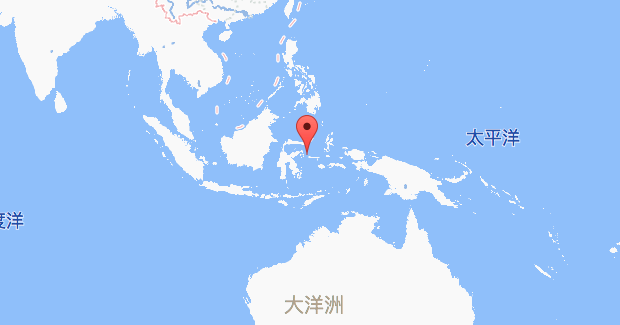
\includegraphics[width=12cm]{q4-yizhi.png}
\caption{地点:帕卢附近} \label{fig:4-yizhi}
\end{figure}


\begin{figure}[!htbp]  
\begin{minipage}[t]{0.5\textwidth}
\centering  
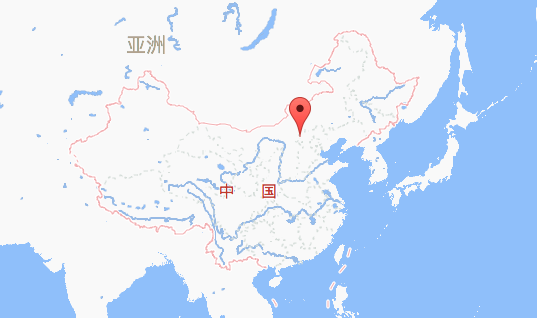
\includegraphics[width=\linewidth]{q4-wei-neimeng.png}
\caption{地点一:内蒙古} \label{fig:q4-wei-neimeng}\end{minipage}
\hspace{1ex}
\begin{minipage}[t]{0.5\textwidth}  
\centering  
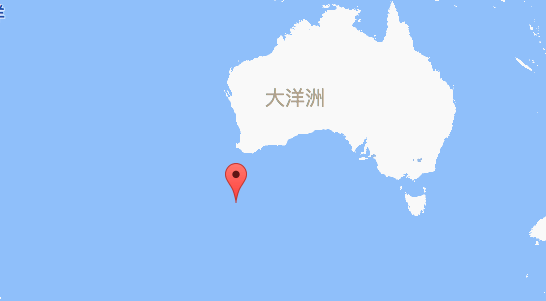
\includegraphics[width=\linewidth]{q4-wei-ao.png}
\caption{地点二:澳大利亚南侧} \label{fig:q4-wei-ao}
\end{minipage}  
\end{figure} 




\newpage
\section{模型优缺点}
\subsection{模型优点}
\begin{enumerate}
	\item 建立最小二乘曲线拟合最优化模型可以通过调整目标函数的取值范围从而得到直杆所在位置的可能结果。
	\item 最小二乘曲线拟合最优化模型考虑了影子长度测量值的误差。
	\item 充分利用地理学方面的知识,求解简单,计算简便。
\end{enumerate}
\subsection{模型缺点}
\begin{enumerate}
	\item 对影长在一天中的长度变化近似认为是抛物线,缺乏进一步证明。
	\item 没有考虑在不同的地理环境,大气对太阳光线的影响。
\end{enumerate}
\section{模型改进方向}
\begin{enumerate}
	\item 对直杆的影子在一天中的长度进行多项式拟合,利用最小二乘确定离差平方和最小时的影长在一天中的变化规律。
	\item 在影长模型计算中加入大气折射对实际太阳高度角的影响。
\end{enumerate}




%参考文献
\begin{thebibliography}{9}%宽度9
 \bibitem{q1-1} 安雨晨, 王兴福, 楚康帅,等. 直杆影子长度随太阳移动的变化曲线的建立[J]. 建筑工程技术与设计, 2016(7).
 \bibitem{时角} \url{https://baike.baidu.com/item/时角/2116855?fr=aladdin}
 \bibitem{赤纬角} \url{https://baike.baidu.com/item/黄赤交角/979385?fr=aladdin&fromid=11324443&fromtitle=太阳赤纬角}
 \bibitem{高度角} \url{https://baike.baidu.com/item/太阳高度角/1563831?fr=aladdin}
\end{thebibliography}

\end{document} 